\documentclass[11pt]{article}
\usepackage{geometry}                
\geometry{letterpaper}                   

\usepackage{url}
\usepackage{listings}
\usepackage{graphicx}
\usepackage{amssymb}
\usepackage{epstopdf}
\usepackage[numbers]{natbib}
\usepackage{amssymb, amsmath}
\usepackage{array}
\usepackage{pdfpages}
\usepackage{float}
\usepackage{caption}
\usepackage{subcaption}
\usepackage{color}


\DeclareGraphicsRule{.tif}{png}{.png}{`convert #1 `dirname #1`/`basename #1 .tif`.png}

%\title{Title}
%\author{Name 1, Name 2}
%\date{date} 

\begin{document}



\thispagestyle{empty}

\begin{center}

\includegraphics[width=5cm]{ETHlogo.eps}

\bigskip


\bigskip


\bigskip


\LARGE{ 	Lecture with Computer Exercises:\\ }
\LARGE{ Modelling and Simulating Social Systems with MATLAB\\}

\bigskip

\bigskip

\small{Project Report}\\

\bigskip

\bigskip

\bigskip

\bigskip


\begin{tabular}{|c|}
\hline
\\
\textbf{\LARGE{Modeling of a passenger ship evacuation}}\\
\textbf{\LARGE{}}\\
\\
\hline
\end{tabular}
\bigskip

\bigskip

\bigskip

\LARGE{Manuela Eugster \& Andreas Reber \& Raphael Brechbuehler \& Fabian Schmid }



\bigskip

\bigskip

\bigskip

\bigskip

\bigskip

\bigskip

\bigskip

\bigskip

Zurich\\
November 2012\\

\end{center}



\newpage

%%%%%%%%%%%%%%%%%%%%%%%%%%%%%%%%%%%%%%%%%%%%%%%%%

\newpage
\section*{Agreement for free-download}
\bigskip


\bigskip


\large We hereby agree to make our source code for this project freely available for download from the web pages of the SOMS chair. Furthermore, we assure that all source code is written by ourselves and is not violating any copyright restrictions.

\begin{center}

\bigskip


\bigskip


\begin{tabular}{@{}p{3.3cm}@{}p{6cm}@{}@{}p{6cm}@{}}
\begin{minipage}{3cm}

\end{minipage}
&
\begin{minipage}{6cm}
\vspace{2mm} \large Manuela Eugster
\end{minipage}

\bigskip
\bigskip
\begin{minipage}{6cm}
\vspace{2mm} \large Raphael Brechbuehler
\end{minipage}
&
\begin{minipage}{6cm}
\vspace{2mm}\large Andreas Reber
\end{minipage}

\bigskip
\bigskip

\begin{minipage}{6cm}
\vspace{2mm} \large Fabian Schmid

\end{minipage}
\end{tabular}


\end{center}
\newpage

%%%%%%%%%%%%%%%%%%%%%%%%%%%%%%%%%%%%%%%

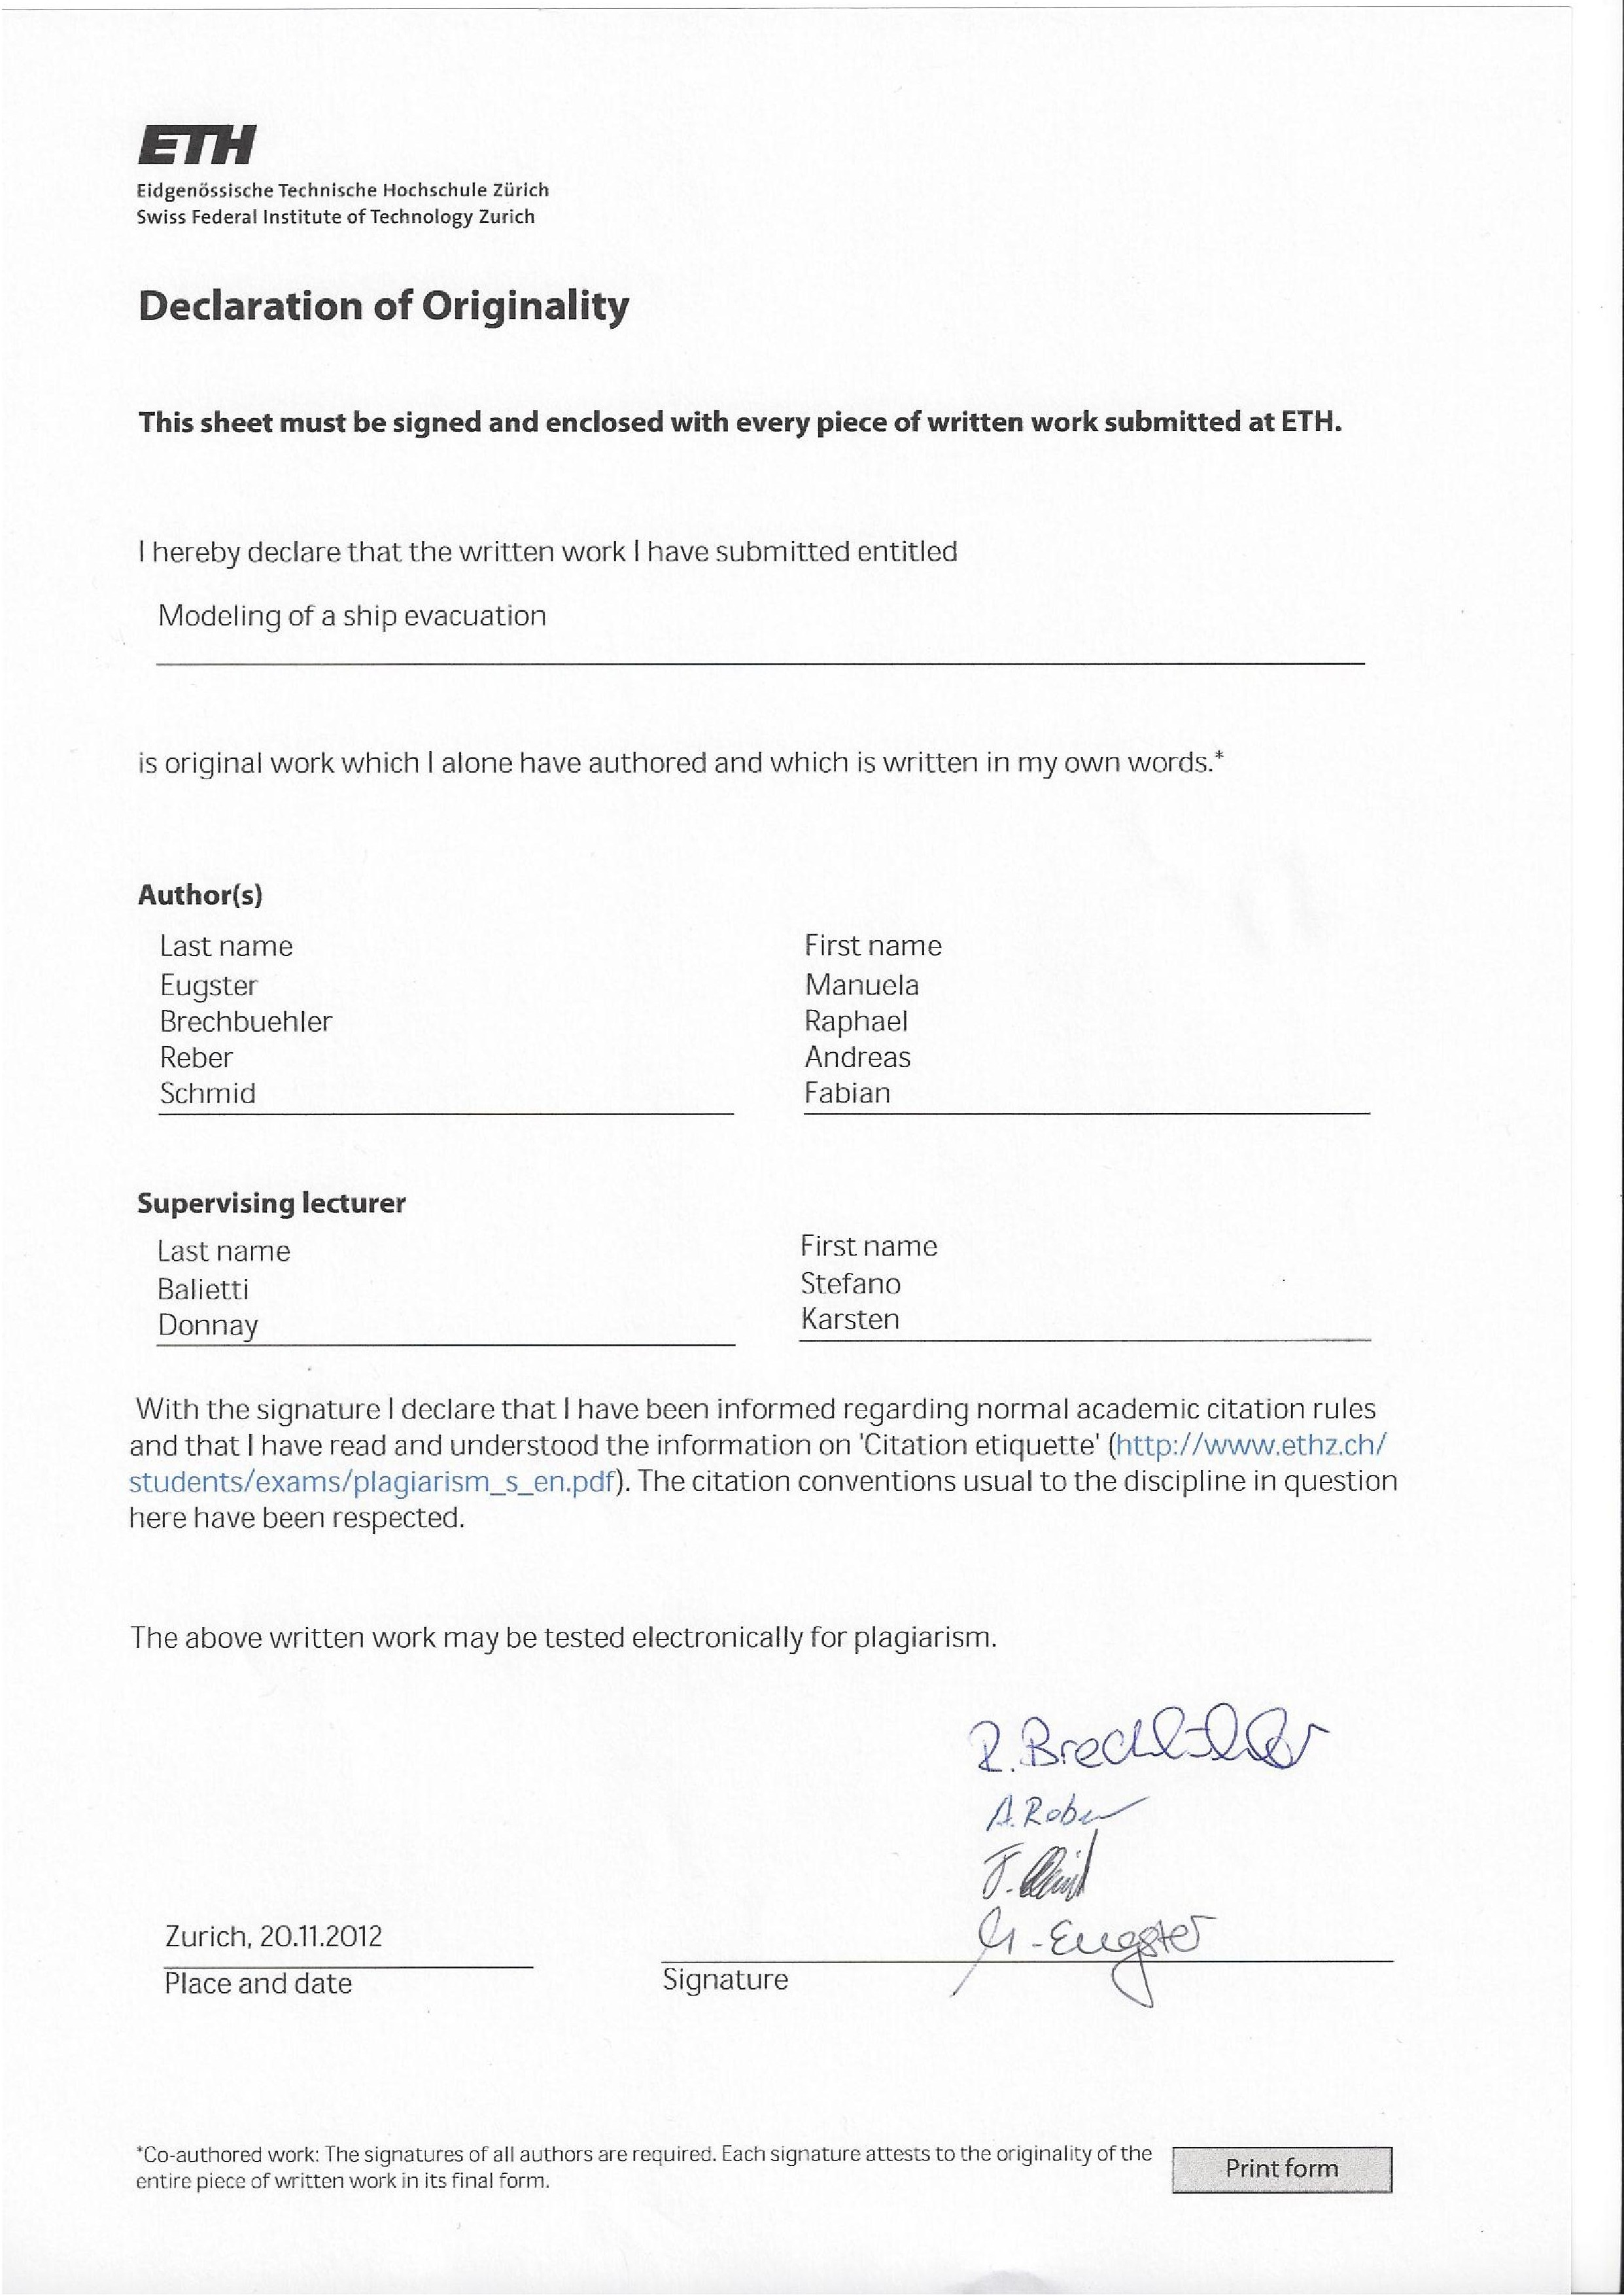
\includegraphics[width=\textwidth]{declaration.jpg}

% IMPORTANT
% you MUST include the ETH declaration of originality here; it is available for download on the course website or at http://www.ethz.ch/faculty/exams/plagiarism/index_EN; it can be printed as pdf and should be filled out in handwriting


%%%%%%%%%% Table of content %%%%%%%%%%%%%%%%%

\tableofcontents

\newpage

%%%%%%%%%%%%%%%%%%%%%%%%%%%%%%%%%%%%%%%



\section{Abstract}

\section{Individual contributions}
The whole project was completed as a team. For sure we took into consideration all the personal backgrounds and  knowledge. That is the reason why Raphael and Manuela focused on implenting the computer code. Whereas Andreas and Fabian concentrated on providing background information, compared the results with the reality and doing its verification.
\section{Introduction and Motivations}
\subsection{Introduction}
The evacuation of a passenger liner due to fire, sinking or other issues leads to several problems. A large amount of passengers try to safe their lives and get to a rescue boat. Narrow and branched floors, smoke, inflowing water, the absence of illumination, rude passengers and so forth can make the evacuation difficult and reduce the number of survivors.
There are a lot of norms how to minimize the harm of such an evacuation. For example there are rules on the number of rescue boats dependent on the amount of passengers \cite{SOLAS}. With dry runs the staff is prepared for the case of emergency et cetera. In real life ship corridor reproduction, the behavior of distressed people is studied.
Another approach is to model such ship evacuations numerically on the computer. As an example the software maritimeEXODUS by a development team from the University of Greenwich is a PC based evacuation and pedestrian dynamics model that is capable of simulating individual people, behaviour and vessel details. The model includes aspects of people-people, people-structure and people-environment interaction. It is capable of simulating thousands of people in very large ship geometries and can incorporate interaction with fire hazard data such as smoke, heat and toxic gases and angle of heel” \cite{EXODUS}.
Our approach is similarly to model a passenger ship with a common geometrical outline and ground view. In an optimization process we will thereafter look for an ideal ground view, rescue boat distribution and their size to minimize the time needed for evacuation. Finally we will make a statement on possible improvements.
\newpage
\subsection{Motivation}
Even though modern ocean liners are considered to be safe, the latest occasions attested that there is still potential for evacuation and safety improvements \cite{concordia}. Certainly we know that this science is very advanced and practised since the sinking of the Titanic. Nevertheless knowing that there are still bottlenecks on the ships we are very motivated to detect and eliminate them with our mathematical models.

\subsection{Fundamental Questions}
To find these bottlenecks we run a mathematical model of a ship structure  with several decks and its passengers \cite{shipdecks}. After we localised these places we are interested in the answers of the following questions:

\bigskip
How much time can be saved by varying the dependent variables mentioned below:
\begin{itemize}
\item How much people can be saved by changing the disposition of the specific room types?
\item Where are the bottlenecks during the evacuation? How can they be avoided?
\end{itemize}

What is the influence of the rescue boats?
\begin{itemize}
\item Are small or bigger boats better?
\item Where do they have to be positioned?
\end{itemize}
If we have time to spare we analyse the difference between uncontrolled and controlled passenger flow:
\begin{itemize}
\item Is the crew able to prevent chaos in the evacuation process?
\item What is the best way to lead the passengers out of the ship?
\end{itemize}
In addition we are keen to know if our model is a good abstraction of the reality?
\section{Description of the Model}
We will base the modeling part on the work done by a group of former "MSSSM" students, by name Hans Hardmeier, Andrin Jenal , Beat Kueng and Felix Thaler. \cite{Building} In their work "Modeling Situations of Evacuation in a Multi-level Building" they wrote a computer program in c with a MATLAB surface to rapidly simulate the evacuation of multi-level buildings.\bigskip
\subsection{Social Force Model }
The simulation is based on the social force model for pedestrian dynamics introduced by Dirk Helbling and Peter Molnar \cite{Helbling}.
The general idea is that a pedestrian can be represented by a particle of a certain mass. Depending on the specific problem, there are defined forces acting on this particle. Due to these forces the particle  moves with a certain speed and velocity in a defined direction.
In our model the following forces are acting on an agent: 
\begin{itemize}
\item $f_{D}$, pulls the agent into the desired direction
\item $f_{ij}$ repulsive forces, keeps a certain distance between agent $i$ and agent $j$
\item $f_{iW}$ wall force, prevents agents $i$ from running into walls
\end{itemize}
For each timestep in the simulation, the forces acting on agent $i$ are calculated. 
Knowing the forces, we can calculate the change in velocity at this timestep:
\begin{equation}
m_{i}\frac{\mathsf{d}\mathbf{v}_{i}}{\mathsf{d}t}=m_{i}f_{D}+\sum \limits_{j(\neq{i})}{f_{ij}}+\sum \limits_{W}{f_{iW}}
\end{equation}
Finally, knowing the change in position the new position can be calculatet:
\begin{equation}
\mathbf{r}_{i,new}=\mathbf{r}_{i,previous}+\mathbf{v}_{i}\mathbf{dt}
\end{equation}
For more detailed information about the forces and their implementation please refer to \cite{Building}chapter 4.

\subsection{General Model}
Similar to the building we necessarily need an  implementation of a common ship shape \cite{shipdecks}. In order to make strong conclusions we want to keep the following variables independent:
\begin{itemize}
\item Number of passengers (4400 agents)
\item Overall capacity of the rescue boats (4680 seats)
\item Ship size and shape
\item Area used by specific rooms (coaches for passengers, lounge area, corridors)
\end{itemize}
Our target is to decrease the evacuation time. Measurements will be made on the time to evacuate:
\begin{itemize}
\item 10\%
\item 50\%
\item 90\%
\item 99\% of all passengers.
\end{itemize}
In order to optimize the evacuation time, we change the following dependent variables:
\begin{itemize}
\item Disposition of the specific room types (e.g. changing the geometry of the corridors without changing the total area used for corridors)
\item Rescue boat size, number and position
\item Control of the passenger flow by crew members (e.g. is there staff to lead the passengers and how are they doing it?)
\end{itemize}

\subsection{Force Model}


\section{Implementation}
\subsection{Code}
As mentioned above our code is based on the work of a previous project. In order to answer our qestion we had to make several adjustments and adapt it to our simulation model. In this chapter we are going to explain the most significant changes. For the exact understanding of the original code and the process of optimization, please refer to the documentation of the previous project group, especially chapter five and nine\cite{Building} or our code in the Appendix.
\subsubsection{Code adjustment - Exits}
\underline{Reason:}
\newline
The first change which was necessary was due to the fact that the exits in our simulation are not simply on the lowest floor.
\newline
\underline{Assumption:}
\newline
In the case of an emergancy all agents are keen to leave the ship as fast as possible. Therefore in our simulation all passangers above the exits floor are only enabled to move down and passengers lower than the exit floor move upstairs.
\newline
\underline{Function:}
\newline
applyForcesAndMove.m
\newline
\underline{New variables:}
\newline 
To define the floor in which the exits are we introduced a new variable \textit{floor\underline{ }exit} in the config file.
\newline
\underline{Modifications:}
\newline
Since we defined our exit, we are able to easily modify the by splitting the loop, in which we calculate the forces and moves of the agents, in two parts. First we loop over all floors higher than the exit floor in which the agents only are allowed to move down or take an exit. Secondly we do the same for all people in the floors lower than the exit floor where the passengers only can move up or take an exit.
\newline
Because of this modification it is not necessary to loop twice over all floors. Consequently our code remains fast and efficient. We also kept the simple concept of vectors out of booleans. Means for each agent there is one number set: If the agent reaches a staircase and therefore changes the floor he is a 1 otherwise he is a 0. The assumption also is a great simplification for the pictures since we do not have to mess with the problem of having overlapping stairs.

\subsubsection{Code adjustment - Different exits}
\underline{Reason:}
\newline
Because the exits model rescueboats, which can only hold a limited number of agents, we were forced to find a way how to differ the exits from each other and to assign a specific number to every exit.
\newline
\underline{Function:}
\newline
loadConfig.m
\newline
\underline{New variables:}
\newline
- \textit{Exit\underline{ }count}, to define the number of exit.\newline
- For each exit k: \textit{exit\underline{ }k\underline{ }nr}, to define the number of agents it can hold.\newline
- To store how many agents can exit in one specific exit, we introduced a matrix exit\underline{ }nr matrix, where the number of agents that can exit is indicated for each pixel.
\underline{Modifications:}
\newline 
We had to make some changes in the decoding of the pictures. The aim was to change as little as possible to the original code. It was clear that we are going to need as many different colors as we have exits, to be able to distinguish them during the simulation.By defining every pixel which is red to value=0, blue value=0 and green value unequal to zero, we can define a lot of different colored exits by using green values from 256 to 256-\textit{exit\underline{ }count}.
\newline
We implemented the matrix \textit{exit\underline{ }nr} similar to the already existing one \textit{img\underline{}exit}, in which we store a count to number the different exits. The number is defined by the green value of  the pixel we are at.

\begin{figure}[h]
\centering
\begin{tabular}
{|>{\large}m{\textwidth}|} \hline
\bigskip
\textcolor{green}{\%make a zeros matrix as big as img\underline{ }exit}
\newline
config.exit\underline{ }nr=zeros(size(config.floor(config.floor\underline{ }exit).img\underline{ }exit));
\newline
\textcolor{green}{\% build the exit\underline{ }nr matrix}
\newline
config.exit\underline{ }nr = config.exit\underline{ }nr + e*( img\underline{ }build(:, :, 1) == 0 \& img\underline{ }build(:, :, 2) == (256-e) \& img\underline{ }build(:, :, 3) == 0 ) ;
\bigskip
\\ \hline
\end{tabular}
\caption{Implementation of the exit\underline{ }nr matrix}
\end{figure}
\subsubsection{Code adjustment - Closing exits during simulation}

\underline{Reason:}
\newline
To close an exit as soon as it let a specific number of agents in, we have to keep track of the number of agents that already used this exit.
\newline
\underline{Function:}
\newline
loadConfig.m and applyForcesAndMove.m
\newline
\underline{New variables:}
\newline 
exit\underline{ }left
\newline
\underline{Modifications:}
\newline
For this purpose, we defined the matrix exit\underline{ }left, in which we store the number of agents who can exit for every exit (defined by his number).

\begin{figure}[H]
\centering
\begin{tabular}
{|>{\large}m{\textwidth}|} \hline
\bigskip
\textcolor{green}{\%make a zeros vector as long as exit\underline{ }count}
\newline
config.exit\underline{ }left = zeros(1,config.exit\underline{ }count);
\newline
\textcolor{green}{\%loop over all exits}
\newline
\textcolor{blue}{for} e=1:config.exit\underline{ }count
\newline
\textcolor{green}{\%build the exit\underline{ }nr matrix}
\newline
config.exit\underline{ }nr = config.exit\underline{ }nr + e*( img\underline{ }build(:, :, 1) == 0 \& img\underline{ }build(:, :, 2) == (256-e) \& img\underline{ }build(:, :, 3) == 0 ) ;
\newline
\textcolor{green}{\%build the exit\underline{ }left matrix}
\newline
config.exit\underline{ }left(1,e) = config.(sprintf(\textcolor{magenta}{'exit\underline{ }\%d\underline{ }nr'}, e)); save the number of agents the exit can hold
\newline
\textcolor{blue}{end}
\bigskip
\\ \hline
\end{tabular}
\caption{Implementation of the exit\underline{ }left matrix}
\end{figure}

\bigskip
In the loop where the forces are calculated and the agents moved, (in function apllyForcesandMove.m) we added a piece of code, which updates the exit\underline{ }left matrix at every time-step.
\newline
First, we get the number of the current exit.

\begin{figure}[h!]
\centering
\begin{tabular}
{|>{\large}m{\textwidth}|} \hline
\bigskip
\textcolor{green}{\%save current exit nr}
\newline
data.current\underline{ }exit = data.exit\underline{ }nr(round(newp(1)), round(newp(2)));
\bigskip
\\ \hline
\end{tabular}
\caption{Implementation to get the current exit number}
\end{figure}

Then we update the exit\underline{ }left matrix by counting down the number of agents allowed to exit by 1. 

\begin{figure}[h!]
\centering
\begin{tabular}
{|>{\large}m{\textwidth}|} \hline
\bigskip
\textcolor{green}{\%update exit\underline{ }left}
\newline
data.exit\underline{ }left(1,data.current\underline{ }exit) = data.exit\underline{ }left(1,data.exit\underline{ }nr(round(newp(1)), round(newp(2)))) - 1;
\bigskip
\\ \hline
\end{tabular}
\caption{Implementation to update the exit\underline{ }left}
\end{figure}

If the allowed number of agents exited the number is 0. Now we have to close the current exit, by changing it into a wall. Therefore we have to update the img\underline{ }wall matrix.

\begin{figure}[h!]
\centering
\begin{tabular}
{|>{\large}m{\textwidth}|} \hline
\bigskip
\textcolor{green}{\%close exit if there is no more free space}
\newline
\textcolor{blue}{if} data.exit\underline{ } left(1,data.current\underline{ }exit) $<$ 1
\newline
\textcolor{green}{\%change current exit to wall}
\newline
data.floor(data.floor\underline{ }exit).img\underline{ }wall = data.floor(data.floor\underline{ }exit).img\underline{ }wall == 1 \textcolor{blue}{...}
\newline
| (data.exit\underline{ }nr == (data.current\underline{ }exit));
\newline
data.floor(data.floor\underline{ }exit).img\underline{ }exit = data.floor(data.floor\underline{ }exit).img\underline{ }exit == 1 \textcolor{blue}{...}
\newline
\& (data.exit\underline{ }nr \~ = (data.current\underline{ }exit));
\bigskip
\\ \hline
\end{tabular}
\caption{Implementation to close filled  boats}
\end{figure}

\subsubsection{Code adjustment - Controlled evacuation}

\underline{Reason:}
\newline
With the goal of a faster evacuation, we tried to control the agents to go to specific exits. 
\newline
\underline{Assumption:}
\newline
We realised that the biggest problem-zones are the stairs. So, in order to get the agents as fast as possible away from the stairs, once they changed the floor, we decided to split the agents in two groups. 
One group only reaches one half of the exits and the other group for the others. 
\newline
\underline{Function:}
\newline
init\underline{ }agents.m, addDesiredForce.m, initEscapeRoutes\underline{ }even.m, initEscapeRoutes\underline{ }odd.m, addDesiredForce.m, initialize.m, initAgents.m, loadConfig.m
\newline
\underline{New variables:}
\newline 
- \textit{numbr}, each agents gets a number ( 0 or 1, selected randomly)
\newline
- \textit{control\underline{ }exit}, in the config file you can decide whether or not you want to have controlled exits during your simulation
\newline
\underline{Modifications:}
\newline
Essentially, we had to modify the calculation of the force dragging a specific agent to the nearest exit.  Therefore we wrote two new functions to init the escape routes. 
\newline
- initEscapeRoutes\underline{ }even.m, this function only considers the exits  which are identified by an even number.

\begin{figure}[H]
\centering
\begin{tabular}
{|>{\large}m{\textwidth}|} \hline
\bigskip
temp1=double(mod(data.exit\underline{ }nr,2)); \textcolor{green}{\%matrix in which every number which is even turns to zero, odd turns to one}
\newline
temp2=logical((data.floor(i).img\underline{ }exit)-(temp1));
\newline
boundary\underline{ }data(temp2)=-1; \textcolor{green}{\%boundary\underline{ }data considers only the exits with even numbers $-->$ -1 }
\bigskip
\\ \hline
\end{tabular}
\caption{Implementation to init escape routes for even numbers}
\end{figure}

$\rightarrow$ initEscapeRoutes\underline{ }.m, this function only considers the exits which are identified by an odd number

\begin{figure}[H]
\centering
\begin{tabular}
{|>{\large}m{\textwidth}|} \hline
\bigskip
temp=logical(mod(data.exit\underline{ }nr,2)); \textcolor{green}{\%matrix in which every number which is even turns to zero, odd turns to one}
\newline
boundary\underline{ }data(temp)=-1; \textcolor{green}{\%boundary\underline{ }data considers only the exits with odd numbers}
\bigskip
\\ \hline
\end{tabular}
\caption{Implementation to init escape routes for odd numbers}
\end{figure}

This as a basis we got two different directions to the next exit.

\begin{figure}[H]
\centering
\begin{tabular}
{|>{\large}m{\textwidth}|} \hline
\bigskip
$\rightarrow$[data.floor(i).img\underline{ }dir\underline{ }x\underline{ }odd, data.floor(i).img\underline{ }dir\underline{ }y\underline{ }odd]
\newline
$\rightarrow$[data.floor(i).img\underline{ }dir\underline{ }x\underline{ }even, data.floor(i).img\underline{ }dir\underline{ }y\underline{ }even]
\bigskip
\\ \hline
\end{tabular}
\caption{Functions used to get the forces which drag the agents to the nearest exit}
\end{figure}

The agents are splitted in “even-agents” and “odd-agents” defined by the randomly added number (0 or 1).

\begin{figure}[H]
\centering
\begin{tabular}
{|>{\large}m{\textwidth}|} \hline
\bigskip
\textcolor{green}{\%even agents}
\newline
\textcolor{blue}{if} numbr==0;
\newline
\textcolor{green}{\%get direction towards nearest exit}
\newline
ex = lerp2(data.floor(fi).img\underline{ }dir\underline{ }x\underline{ }even, p(1), p(2));
\newline
ey = lerp2(data.floor(fi).img\underline{ }dir\underline{ }y\underline{ }even, p(1), p(2));
\newline
e = [ex ey];
\newline
\textcolor{green}{\%get force}
\newline
Fi = m * (v0*e - v)/data.tau;
\newline
\textcolor{green}{\% add force}
\newline
data.floor(fi).agents(ai).f = data.floor(fi).agents(ai).f + Fi;
\newline
\textcolor{blue}{end}
\bigskip
\\ \hline
\end{tabular}
\caption{Implementation to randomly split agents to even and odd}
\end{figure}




\subsection{Ship Decks}
\section{Simulation Results and Discussion}
\subsection{Expected Results}
\begin{itemize}
\item Even though modern ships are quite optimized in regard to evacuation time, they are always a compromise between safety and luxury. Therefore we are convinced to find a superior adjustment of the decks geometries to increase the survival rate.
\item Since the rescue boats can not be averaged but are rather concentrated over one or two decks, we consider the staircases as the bottlenecks.
\item In alinging this variables we are persuaded of a reduction of the overall evacuation time.
\item We suppose that smaller and evenly spread rescue boats combined with a higher quantity will scale the evacuation time down. Certainly there is going to be an optimum in size which we are willing to find.
\item By controlling the rescue we assume to detect a huge decrease in evacuation time. Further we have the hypothesis that disorder can be minimized. The crew who is familiar with the decks and the emergency exits is able to guide the passengers in minimum time to the rescue boats.
\item There are many parameters we do not model in our simulation. For example fire and smoke, the tilt of the ship or handicapped and petrified passengers are disregarded. By leaving out this details we get a very simplified model. However, by starting the optimization process by data of a nowadays passenger liner \cite{shipdecks} we hope to see some real evacuation dynamics in this system and therefore make conclusion on the fundamental questions.
\end{itemize}
\subsection{Simulation Results}
\subsubsection{Standard ship}
As listed above we were interested in the time in which a certain percentage of all agents was evacuated:
\newline

\begin{table}[h]
\centering
\begin{tabular}
{|>{\large}m{2cm} |>{\center}b{1.1cm} |>{\center}b{1.1cm}|>{}b{1.1cm}|>{}b{1.1cm}|} \hline \hline
percentage of agents.& 10\% &  50\% & 90\% &99\% \\ \hline
evacuation time & 69s &272s & 468s & 614s \\ \hline \hline
\end{tabular}
\caption{Standard simulation: Needed time to evacuate a certain percentage of all agents.}
\end{table}

Further our standard ship simulation showed the following performance:

\begin{figure}[htbp]
\centering
{\begin{minipage}[t]{7.4cm}
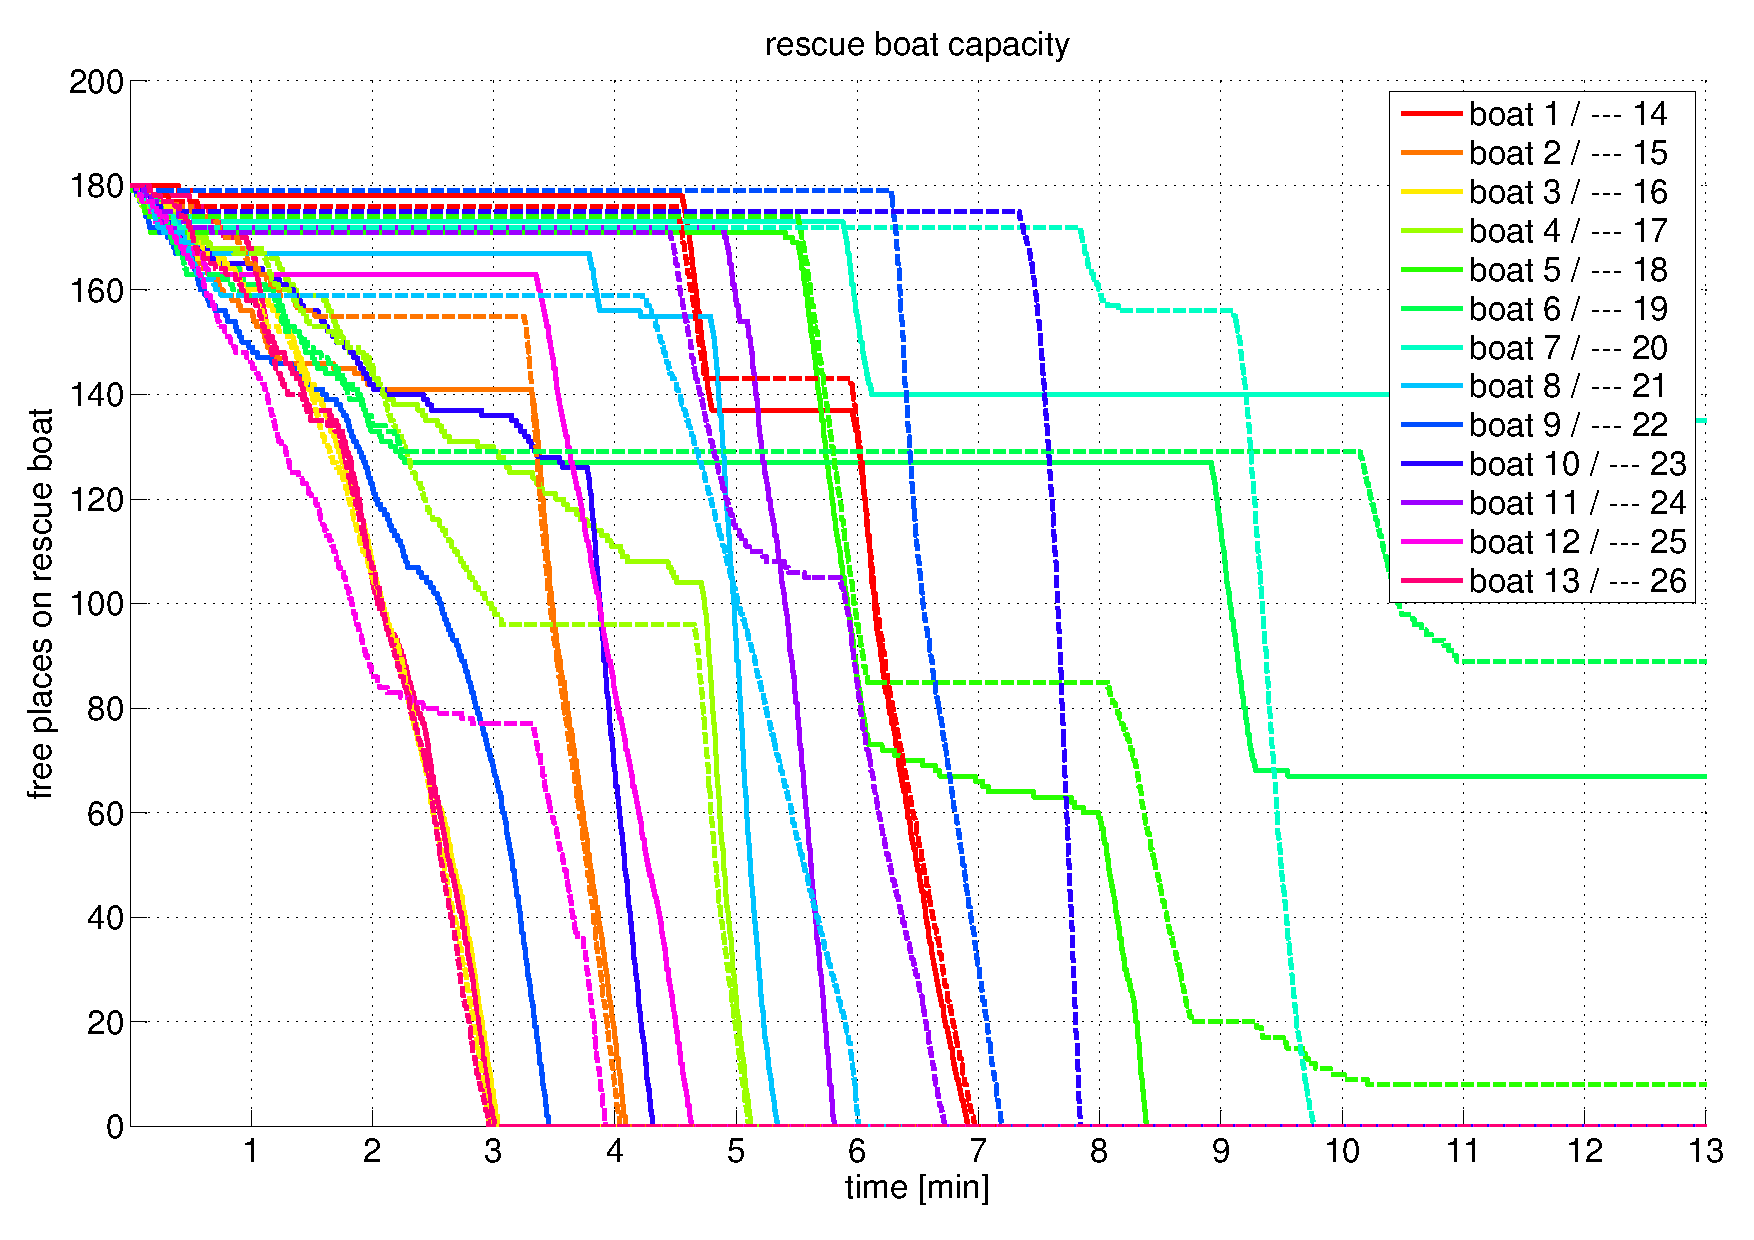
\includegraphics[width=\textwidth]{run1-standard-rescueboatcapacity.pdf}
\caption{Standard simulation: Boat capacities during simulation}
\end{minipage}}
{\begin{minipage}[t]{7.4cm}
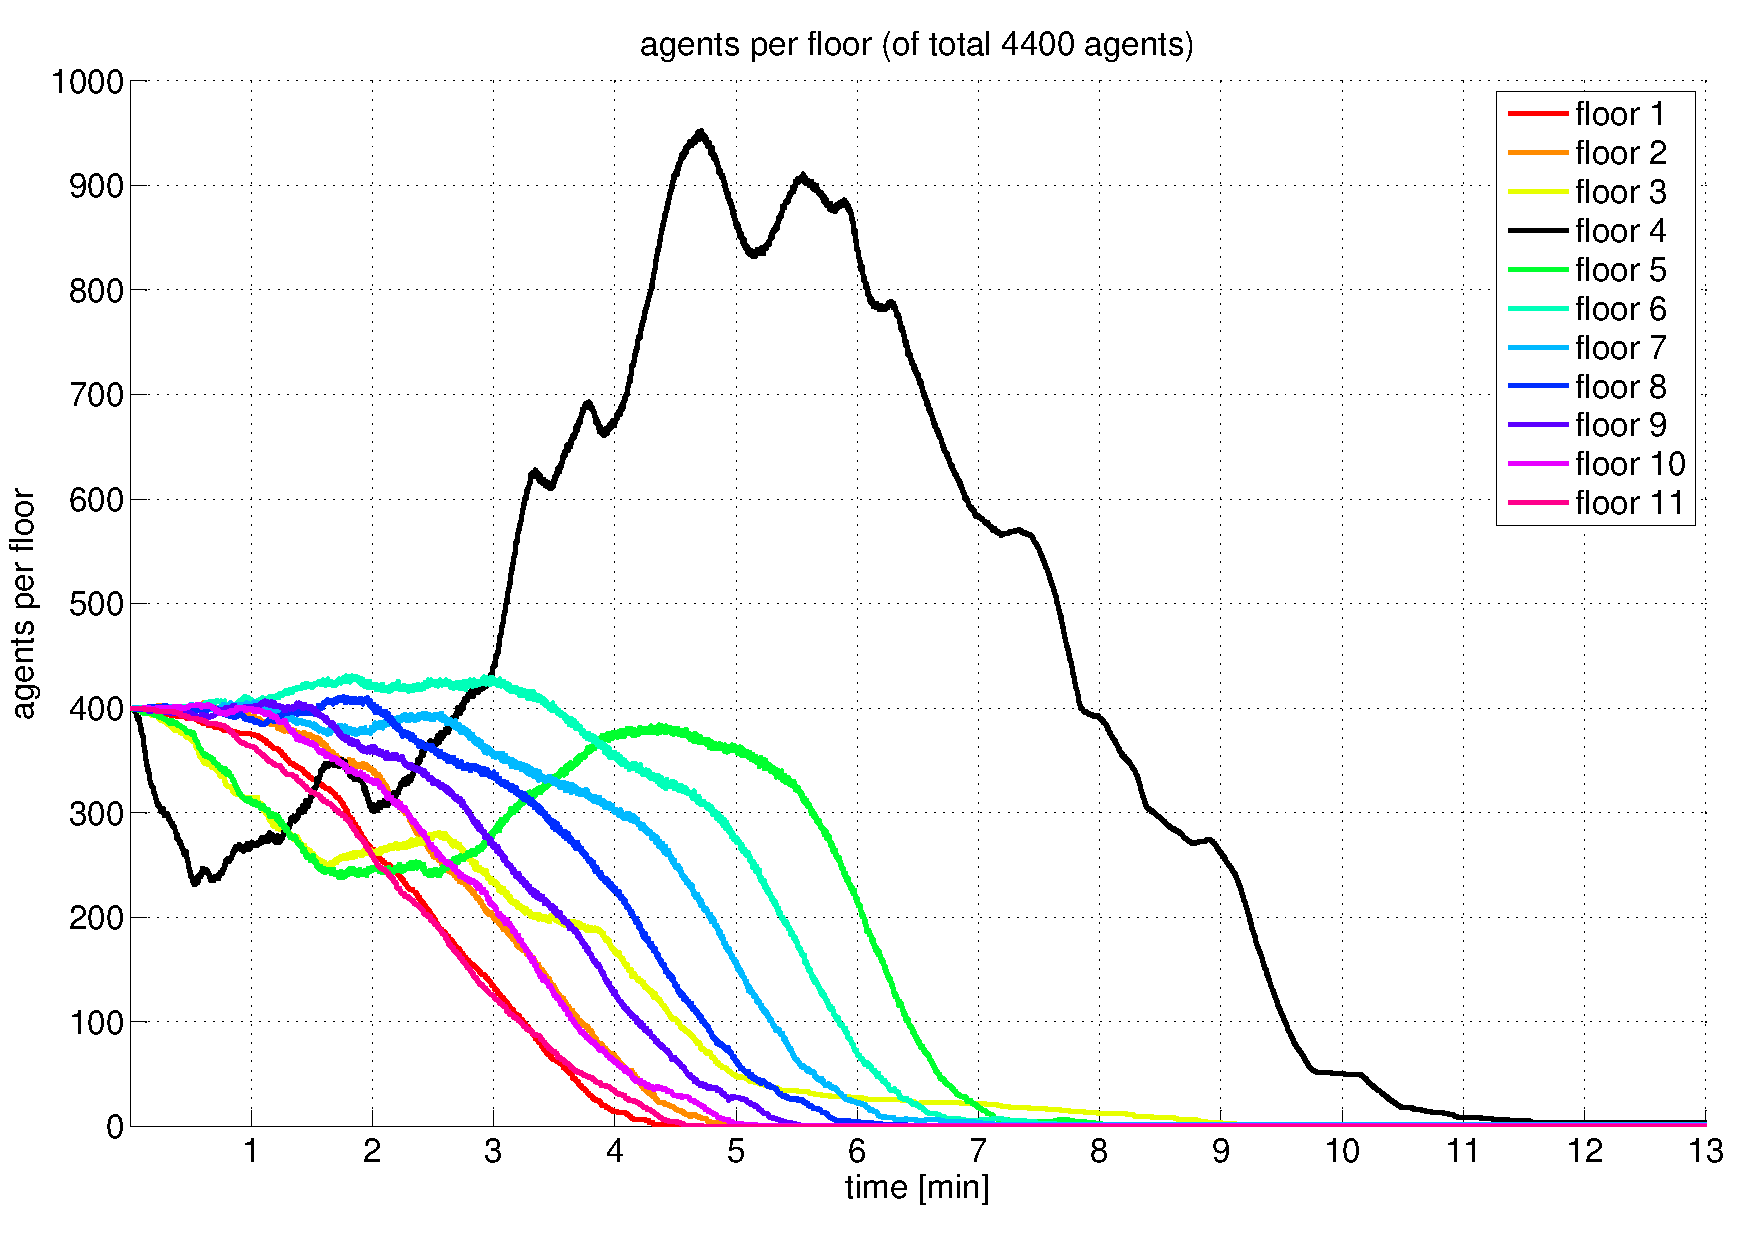
\includegraphics[width=\textwidth]{run1-standard-agentsperfloor.pdf}
\caption{Standard simulation: Number of agents per floor}
\end{minipage}}
\end{figure}

\subsubsection{Modified room disposition}
As we expected the standard simulation revealed that hold-up problems occur because of the staircases. As the flow everywhere else was quite dynamic we abstained from adjusting the room disposition but instead we inserted an additional staircase. This simulation yielded the following results:

\begin{table}[h]
\centering
\begin{tabular}
{|>{\large}m{2cm} |>{\center}b{1.1cm} |>{\center}b{1.1cm}|>{}b{1.1cm}|>{}b{1.1cm}|} \hline \hline
percentage of agents.& 10\% &  50\% & 90\% & 99\% \\ \hline
evacuation time & 72s &259s & 461s & 595s \\ \hline \hline
\end{tabular}
\caption{Added stairs simulation: Needed time to evacuate a certain percentage of all agents.}
\end{table}

\begin{figure}[htbp]
\centering
{\begin{minipage}[t]{7.4cm}
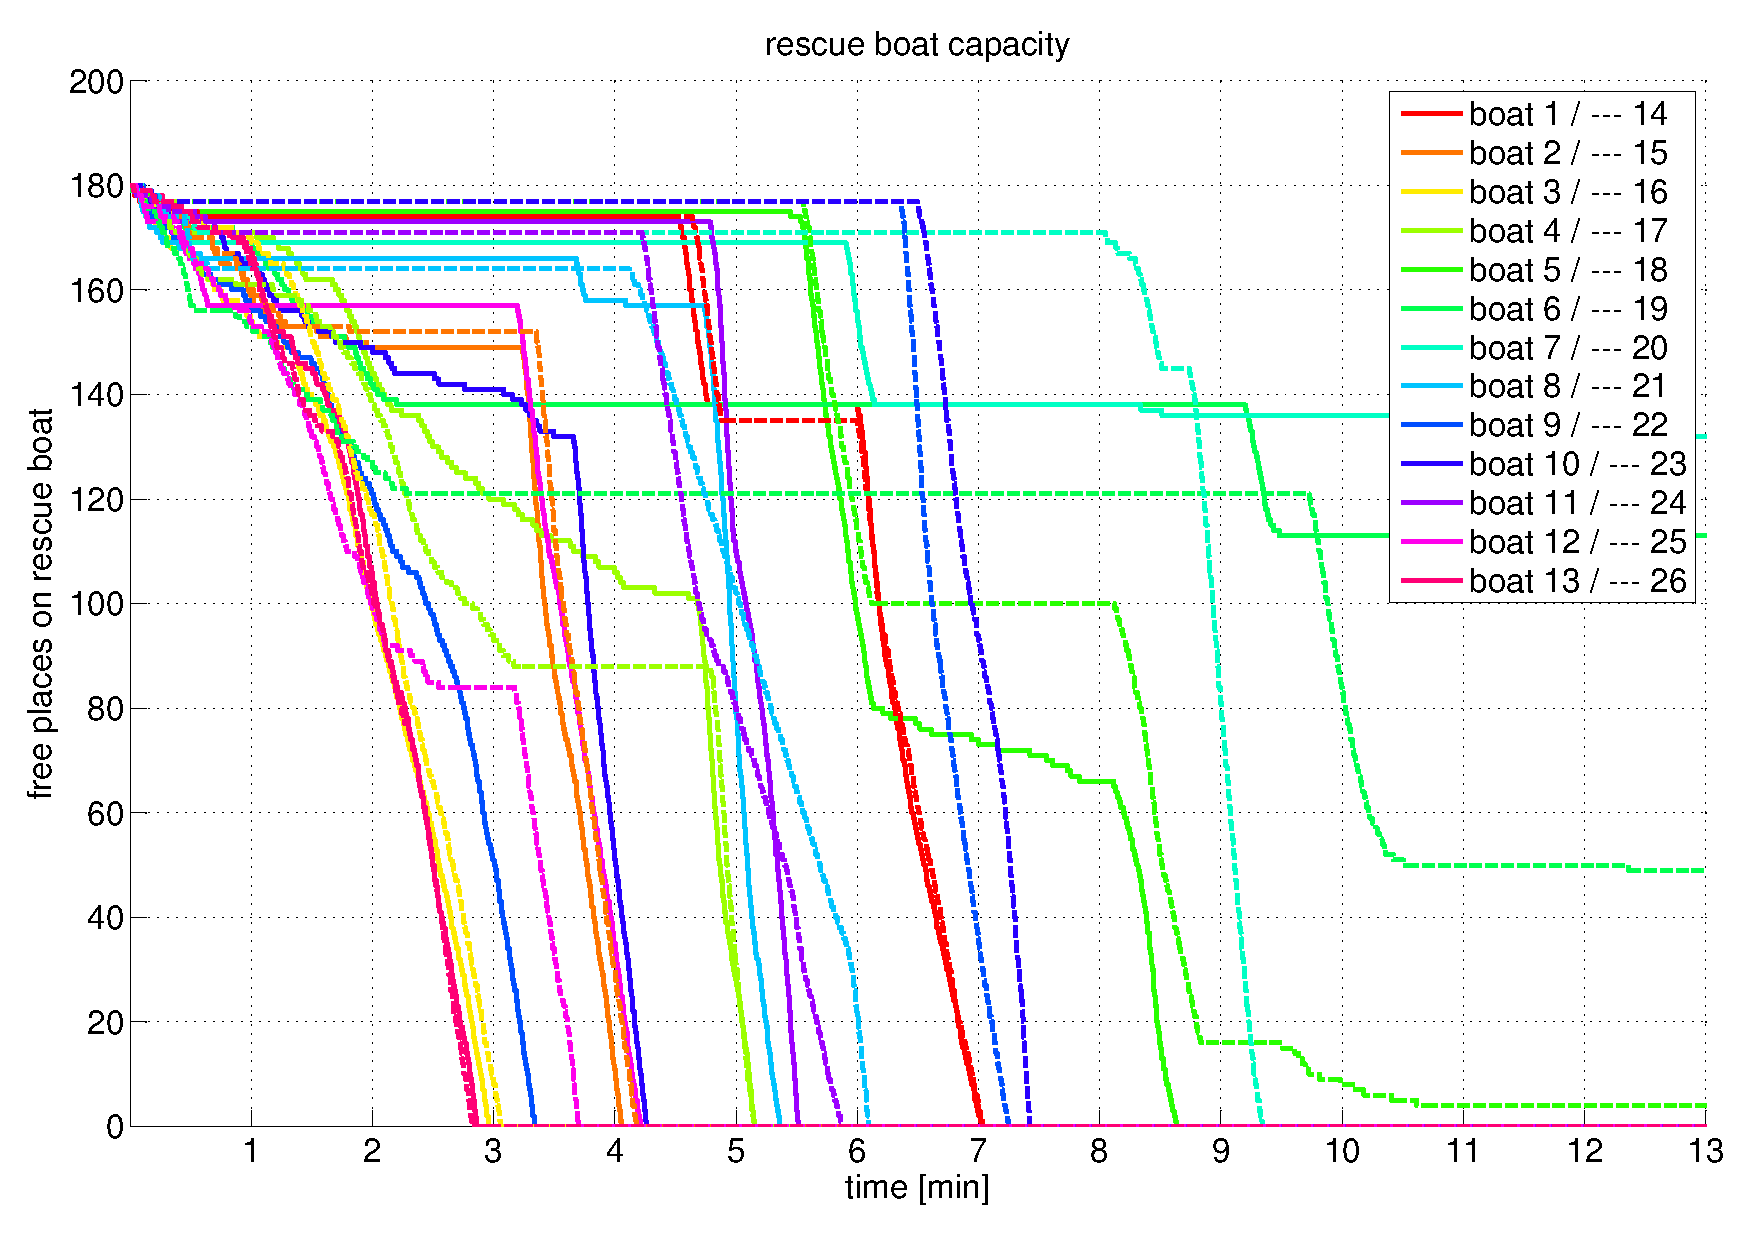
\includegraphics[width=\textwidth]{run1-added-stairs-rescueboatcapacity.pdf}
\caption{Added stairs simulation: Boat capacities during simulation}
\end{minipage}}
{\begin{minipage}[t]{7.4cm}
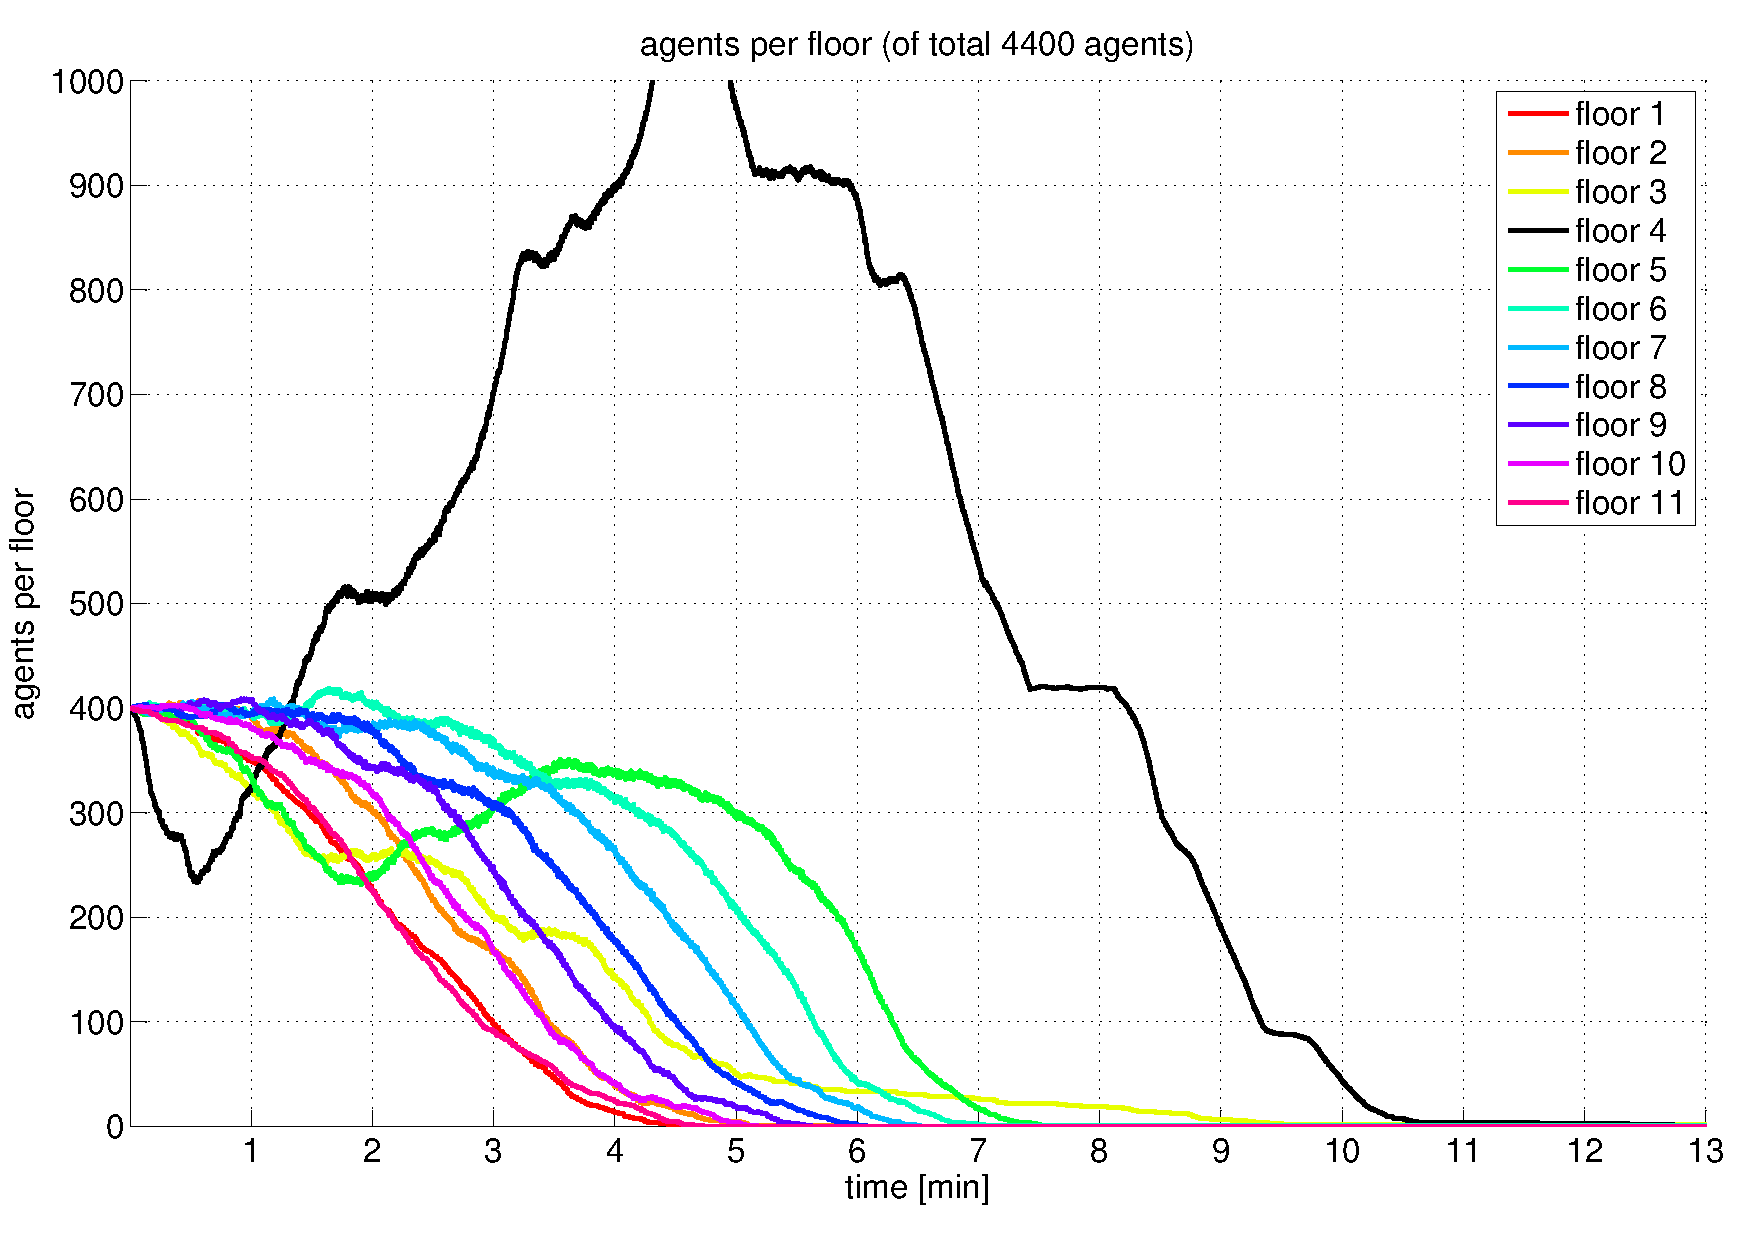
\includegraphics[width=\textwidth]{run1-added-stairs-agentsperfloor.pdf}
\caption{Added stairs simulation: Number of agents per floor}
\end{minipage}}
\end{figure}
 
\subsubsection{Modified rescueboat size}
As we could see in the simulations with the standard ship, the rescueboats which are nearest to the stairs are filled first. This behavior is very intuitive. As soon as the nearest lifeboats are full, the agents continue to fill the other lifeboats. 
The greatest extension of the evacuation time occurs as follows:
Towards the end of the simulation, not all lifeboats are still open. Therefore leftover agents, which walked in the direction of a lifeboat that closed in the meantime,have to cross a big distance to reach a lifeboat with free space.\newline
We tried to avoid this delay by increasing the capacity of the lifeboats near to the stairs and removed some, which are the farthest away for the agents left over towards the end of the evacuation.



\begin{table}[h]
\centering
\begin{tabular}
{|>{\large}m{2cm} |>{\center}b{1.1cm} |>{\center}b{1.1cm}|>{}b{1.1cm}|>{}b{1.1cm}|} \hline \hline
percentage of agents.& 10\% &  50\% & 90\% & 99\% \\ \hline
evacuation time & 71.44s &257.12s & 419.4s & 571.4s \\ \hline \hline
\end{tabular}
\caption{Varied boatsize simulation: Needed time to evacuate a certain percentage of all agents.}
\end{table}



\subsubsection{Crew command}
\subsection{Comparison}
\subsubsection{Standard - Modified room disposition}
The Analysis of the simulation results showed that there is a huge potential in saving evacuation time. By adding just one additional staircase we were able to reduce the overall evacuation time by almost 20 seconds. Further 50\% of all agents entered the exits approximately 13 seconds earlier compared to the stanard model. In contrast to that the rescueboat capacity utilisation remains basically the same. Another point which was actually not important for our research is that you get a much higher agent densitiy on the exit floor. 
\subsubsection{Standard - Modified rescueboat size}

As the results above show, there is no significant acceleration in the first part of the evacuation achieved by changing the distribution of the lifeboats .  
 But, there is clearly a difference in second half of the evacuation. The last 10\% of agents are evacuated 48.6 seconds faster and the last 1\% even 42.6 seconds faster. 
This decrease in evacuation time is an effect of the reduced time the last agents need to leave the exit-deck.


\subsubsection{Standard - Crew command}
\subsection{Discussion}
\section{Summary and Outlook}
\subsection{Summary}
\subsection{Outlook}
During our work on this project, we found a lot of possibilites to improve the model. The target of an ongoing project could be to make the model more realistic. There are a lot of possibilites to achieve this goal.
\newline
Some suggestions:
\begin{itemize}
\item To take into account that not all people automatically know where exactly the nearest exit is, the initialisation of the escape routes should be modified.
\item In our model the agents are evenly distributed over the floors and decks at the beginning of the simulation. This is however a very unrealistic scenario. In reality the agents will be uneavenly spread. The evacuation time would depend very much on the form of this distribution.
\item Different scenarios like night, dinner-time etc. that would change the distribution of the agents significantly could be compared.
\item In reality there are a lot of effects that could occur like fire, tilt of the ship, flooded areas, power failure, mass panic etc.
\end{itemize}
There are a lot of other interesting effects that could be looked at as well.
\\
Some ideas:
\begin{itemize}
\item In the ideal case, the evacuations on a ship are planned well. A good idea would be to define specific control points at which agents gahter first. From those points the agents would be led in small groups to the rescueboats by a crew member. It would be interesting to analyse the effect of such a efficient control.
\item The optimal combination of the different modifications we analyzed in this project could be found and therefore a minimal evacuation time.
\end{itemize}
\section{References}
\begin{thebibliography}{9}
\bibitem{Helbling} Helbing, Dirk (1995): Social Force Model for Pedestrians Dynamics.
\bibitem{Building} Hardmeier,Jenal,Kueng,Thaler (2012): Modelling Situations of Evacuation in a Multi-level Building.
\bibitem{SOLAS} SOLAS (1974): International Convention for the Safety of Life at Sea. \url{http://www.imo.org/about/conventions/listofconventions/pages/international-convention-for-the-safety-of-life-at-sea-(solas),-1974.aspx}
\bibitem{ship} SHIP EVACUATION: \url{http://www.shipevacuation.com/}
\bibitem{shipdecks} CRUISE DECK PLANS PUBLIC SITE: \url{http://www.cruisedeckplans.com/DP/Main/decks.php?ship=Costa%20Serena}
\bibitem{EXODUS} University of Greenwich (2011):  maritimeEXODUS. \url{http://fseg.gre.ac.uk/fire/marine_evac_model.html}
\bibitem{concordia} Haverie of Costa Concordia (2012): \url{http://de.wikipedia.org/wiki/Costa_Concordia#Havarie_2012}
	
\end{thebibliography}
\section{Appendix}
\subsection{Code}

% define colors
\definecolor{commentcolor}{RGB}{89, 168, 89}
\definecolor{keywordcolor}{RGB}{68, 68, 255}
\definecolor{stringcolor}{RGB}{205, 139, 247}
\definecolor{numbercolor}{RGB}{128, 128, 128}
\definecolor{bgcolor}{RGB}{245, 248, 253}

% define listings style
\lstset{
  language=Matlab,
  basicstyle=\footnotesize\ttfamily,
  numbers=left,
  numberstyle=\tiny\color{numbercolor},
  stepnumber=2,
  numbersep=5pt,
  backgroundcolor=\color{bgcolor},
  showspaces=false,
  showstringspaces=false,
  showtabs=false,
  frame=lines,
  rulecolor=\color{black},
  tabsize=2,
  captionpos=b,
  breaklines=true,
  breakatwhitespace=true,
  title=\lstname,
  commentstyle=\color{commentcolor},
  keywordstyle=\color{keywordcolor},
  stringstyle=\color{stringcolor}
}






\end{document}  



 
